%-------------------------------------------
\begin{frame}{RNAseq analysis}
%\againframe<2>{RNAseqWF_diapo}
%-------------------------------------------
\begin{block}{Analysis workflow}
    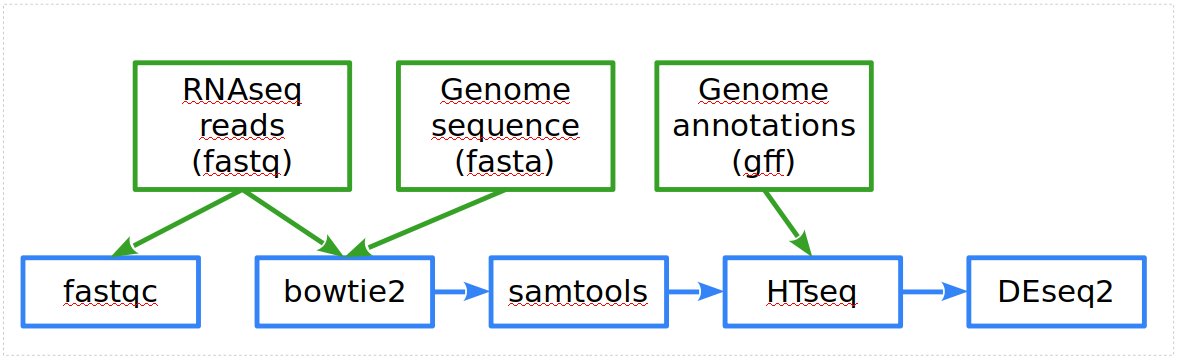
\includegraphics[width=12cm]{01_introduction/images/FAIR_RNAseq_WF.png}\\
green=input, blue=tool
\end{block}
\footnotesize{
\begin{description}
    \item[fastqc] control quality of the input reads
    \item[bowtie2] reads mapping on the genome sequence
    \item[samtools] mapped reads selection $\&$ formatting
    \item[HTseq] count table of mapped reads on genes (annotations)
    \item[DEseq2] statistical analysis: genes list having differential expression
\end{description}
}
\end{frame}
%-------------------------------------------
\begin{frame}[containsverbatim]
\frametitle{Data and command line}
%-------------------------------------------
\begin{exampleblock}{Data}
-g genome sequence acces (including extention .fna, .fasta)\\
-a genome annotation acces (inluding extention .gff)\\
-d RNAseq sample prefix\\
next args: RNAseq sample prefix, no .fastq.gz extention
\end{exampleblock}
\begin{exampleblock}{Bash command line}
\begin{lstlisting}
FAIR_initial_script.sh -g ../O.tauri_genome.fna -a ../O.tauri_annotation.gff -d ../ SRR3099585_chr18 S*86_chr18 S*87_chr18 S*97_chr18 S*98_chr18 S*99_chr18
\end{lstlisting}
\end{exampleblock}
\begin{exampleblock}{Script in 3 main blocks}
\begin{lstlisting}
1) while getops do ... done   
2) for sample in $* ; do ... done   
3) creation of the result file, counts.txt, with paste, awk, and sed bash commands
\end{lstlisting}
\end{exampleblock}
\end{frame}
%-------------------------------------------
\begin{frame}[containsverbatim]
\frametitle{Complete bash script, 1/3}
%-------------------------------------------
\begin{exampleblock}{getops block}
\begin{lstlisting}
while getopts g:a:d: flag do
        case $flag in
            g)  genome=$OPTARG
                echo genome is $genome ;;
            a)  annots=$OPTARG
                echo annotation is $annots ;;
            d)  rnadir=$OPTARG
                echo RNAseq path is $rnadir ;;
            :)  echo "L'option $OPTARG requiert un argument"
                exit 1 ;;
            \?) echo "$OPTARG : option invalide"
                exit 1 ;;
        esac
   done
shift $(( OPTIND - 1 ))  # shift past the last flag or argument
echo samples are $*
\end{lstlisting}
\end{exampleblock}
\end{frame}
%-------------------------------------------
\begin{frame}[containsverbatim]
\frametitle{Complete bash script, 2/3}
%-------------------------------------------
\begin{exampleblock}{for block}
\begin{lstlisting}
nbs=0;
for sample in $* ; do 
   nbs=$(expr ${nbs} + 1)
   echo traitement of sample ${sample}
   # --------- quality control of reads
   if [ ! -d FastQC ]; then
       mkdir FastQC
   fi
   fastqc --outdir FastQC ${rnadir}${sample}.fastq.gz > FastQC/${sample}.log 2>&1
   #---------- reads mapping
   if [ ! -d Bwt2_index ]; then
       mkdir Bwt2_index
       bowtie2-build ${genome} Bwt2_index/tauri > Bwt2_index/Bwt2_index.log 2>&1
   fi
\end{lstlisting}
\end{exampleblock}
\end{frame}
%-------------------------------------------
\begin{frame}[containsverbatim]
\frametitle{Complete bash script, 3/3}
%-------------------------------------------
\begin{exampleblock}{for block, continuation}
\begin{lstlisting}
   bowtie2 -x Bwt2_index/tauri -U ${rnadir}${sample}.fastq.gz -S ${sample}.sam > ${sample}_bowtie2.log 2>&1
   #---------- selection and format modification
   samtools view -b ${sample}.sam -o ${sample}.bam
   samtools sort ${sample}.bam -o ${sample}_sort.bam
   samtools index ${sample}_sort.bam
   #---------- counting of mapped reads by gene
   featureCounts -t gene -g ID -a ${annots} -s 2 -o ${sample}_ftc.txt ${sample}_sort.bam > ${sample}_ftc.log 2>&1
done
\end{lstlisting}
\end{exampleblock}
\begin{exampleblock}{Count table block}
\begin{lstlisting}
paste *_ftc.txt > ftc_tmp.txt
awk -v nb=${nbs} -v col=7 'BEGIN{FS="\t"}{ctmp=$1; for(i=col;i<=nb*col;i=i+col){count=sprintf("%s\t%s",ctmp,$i);ctmp=count};print count}' ftc_tmp.txt | sed 1d > counts.txt
\end{lstlisting}
\end{exampleblock}
\end{frame}
%-------------------------------------------
\begin{frame}[containsverbatim]
\frametitle{Exercise 2}
%-------------------------------------------
Continue the snakefile of the previous exercise in order to replace the bash script. \\
We will:
\begin{exampleblock}{Objectives}
\begin{itemize}
    \item add a configuration file
    \item use a builtin snakemake function to get filenames of the input RNAseq data
    \item add rules to replace the mapping, formatting, counting, and counts aggregating steps of the bash script
\end{itemize}
\end{exampleblock}
\begin{exampleblock}{ex2$\_$o1.smk}
\begin{lstlisting}
cp ex1_o7.smk ex2_o1.smk
\end{lstlisting}
\end{exampleblock}
\end{frame}
%-------------------------------------------
\begin{frame}[containsverbatim]
\frametitle{getops block}
%-------------------------------------------
\begin{exampleblock}{Shell script}
\begin{lstlisting}
while getopts g:a:d: flag do
        case $flag in
            g)  genome=$OPTARG 
            ...
\end{lstlisting}
\end{exampleblock}
We will use a configuration file:
\begin{exampleblock}{Objective 1}
Add a configuration file, named \verb|RNAseq.yml|, containing both the genome sequence and the annotation files manes, and the access to the Data directory. \\
In the snakefile, change the configured variables (ex. replace \verb|Data/| and \verb|genome| by their \verb|config[]| values). The Python strings concatenation is \verb|+|\\
Then, run snakemake with the \verb|--configfile| option.
\end{exampleblock}
\end{frame}
%-------------------------------------------
\begin{frame}[containsverbatim]
\frametitle{Adding a configuration file}
%-------------------------------------------
\begin{exampleblock}{ex2$\_$o1.yml}
\begin{lstlisting}
genome:
  O.tauri.fna
annots:
  O.tauri.gff
dataDir:
  Data/
\end{lstlisting}
\end{exampleblock}
\begin{exampleblock}{ex2$\_$o1.smk: "Data/..." in inputs replaced by a config call:}
\begin{lstlisting}
rule genome_bwt2_index:   config["dataDir"]+config["genome"]
rule fastqc:   config["dataDir"]+"{sample}.fastq.gz"
\end{lstlisting}
\end{exampleblock}
\begin{exampleblock}{snakemake run:}
\begin{lstlisting}
rm -Rf FastQC/ Result/ Tmp/ Logs/ ; snakemake -s ex2_o1.smk --configfile ex2_o1.yml
\end{lstlisting}
\end{exampleblock}
\end{frame}
%-------------------------------------------
\begin{frame}[containsverbatim]
\frametitle{for block}
%-------------------------------------------
\begin{exampleblock}{Shell script}
\begin{lstlisting}
nbs=0;
for sample in $* ; do 
   ...
done
\end{lstlisting}
\end{exampleblock}
To manage all *.fastq.gz files in a directory, use the \verb|glob_wilcards()| function. In \verb|ex2_o2.smk|, replace the SAMPLES definition by:
\begin{exampleblock}{ex2$\_$o2.smk}
\begin{lstlisting}
SAMPLES, = glob_wildcards(config["dataDir"]+"{sample}.fastq.gz")
\end{lstlisting}
\end{exampleblock}
and run snakemake.
\end{frame}
%-------------------------------------------
\begin{frame}[containsverbatim]
\frametitle{Quality control, fastqc}
%-------------------------------------------
\begin{exampleblock}{}
\begin{lstlisting}
if [ ! -d FastQC ]; then
   mkdir FastQC
fi
fastqc --outdir FastQC ${sample}.fastq.gz > FastQC/${sample}.log 2>&1
\end{lstlisting}
\end{exampleblock}
No more need to test the existence of a directory, it is created as needed.
\begin{exampleblock}{rule fastqc:}
This rule is already present in the snakefile
\end{exampleblock}
\end{frame}
%-------------------------------------------
\begin{frame}[containsverbatim]
\frametitle{Reads mapping, bowtie2}
%-------------------------------------------
\begin{exampleblock}{}
\begin{lstlisting}
if [ ! -d Bwt2_index ]; then
   mkdir Bwt2_index
   bowtie2-build ${genome} Bwt2_index/tauri > Bwt2_index/Bwt2_index.log 2>&1
fi
bowtie2 -x Bwt2_index/tauri -U ${sample}.fastq.gz -S ${sample}.sam > ${sample}_bowtie2.log 2>&1
\end{lstlisting}
\end{exampleblock}
2 rules: \verb|genome_bwt2_index| (cf. previous ex.) and \verb|bwt2_mapping|
\begin{exampleblock}{ex2$\_$o3.smk, rule bwt2$\_$mapping (no run):}
\begin{lstlisting}
  output: "results/{sample}.sam"
  input: config["dataDir"]+"{sample}.fastq.gz",
         expand("Tmp/Otauri.{ext}.bt2", ext=BIDX)
  log: "Logs/{sample}_bwt2_mapping.log"
  shell: "bowtie2 -x Tmp/Otauri -U {input[0]} -S {output} 2> {log} "
\end{lstlisting}
\end{exampleblock}
\end{frame}
%-------------------------------------------
\begin{frame}[containsverbatim]
\frametitle{Reads mapping, bowtie2}
%-------------------------------------------
\begin{exampleblock}{Why some troubles?}
The snakemake launch probably didn't do what was expected. 
What have we forgotten? \\
We added a new rule to a snakemake but we didn't manage the rule tree, their is no input-output link to include the new rule to the workflow.\\
We will do that by completing the input directive of the target rule (caution to respect the Python "list" structure, coma-separated).
\end{exampleblock}
\begin{exampleblock}{ex2$\_$o2.smk, target rule:}
\begin{lstlisting}
rule all:
  input:
    expand("FastQC/{sample}_fastqc.html", sample=SAMPLES),
    expand("Tmp/Otauri.{ext}.bt2", ext=BIDX),
    expand("Tmp/{sample}.sam", sample=SAMPLES)
\end{lstlisting}
\end{exampleblock}
\end{frame}
%-------------------------------------------
\begin{frame}[containsverbatim]
\frametitle{samtools}
%-------------------------------------------
\begin{exampleblock}{Shell script}
\begin{lstlisting}
samtools sort -O bam -o ${sample}_sort.bam ${sample}.sam
samtools index ${sample}_sort.bam
\end{lstlisting}
\end{exampleblock}
\begin{exampleblock}{ex2$\_$o4.smk, rule sam2bam$\_$sort (no run):}
\begin{lstlisting}
  output:
    bam="Result/{sample}_sort.bam",
    bai="Result/{sample}_sort.bam.bai"
  input: "Tmp/{sample}.sam"
  log:
    sort="Logs/{sample}_sam2bam_sort.log",
    index="Logs/{sample}_bam2bai.log"
  shell: 
    "samtools sort -O bam -o {output.bam} {input} 2> {log.sort} ;"
    "samtools index {output.bam} 2> {log.index}"
\end{lstlisting}
\end{exampleblock}
\end{frame}
%-------------------------------------------
\begin{frame}[containsverbatim]
\frametitle{FeatureCount}
%-------------------------------------------
\begin{exampleblock}{Shell script}
\begin{lstlisting}
featureCounts -t gene -g ID -a ${annots} -s 2 -o ${sample}_ftc.txt ${sample}_sort.bam > ${sample}_ftc.log 2>&1
\end{lstlisting}
\end{exampleblock}
\begin{exampleblock}{ex2$\_$o5.smk, rule counting (params; no run):}
\begin{lstlisting}
  output: "Tmp/{sample}_ftc.txt"
  input:
    bam="Result/{sample}_sort.bam",
    annot=config["dataDir"]+config["annots"]
  params: t="gene", g="ID", s="2"
  log: "Logs/{sample}_counts.log"
  shell: "featureCounts -t {params.t} -g {params.g} -a {input.annot} -s {params.s} -o {output} {input.bam} &> {log}"
\end{lstlisting}
\end{exampleblock}
\end{frame}
%-------------------------------------------
\begin{frame}[containsverbatim]
\frametitle{Counts matrix creation}
%-------------------------------------------
\begin{exampleblock}{Shell script}
\begin{lstlisting}
paste *_ftc.txt > counts_tmp.txt
awk -v nb=${nb_sample} 'BEGIN{FS="\t"}{count_tmp=$1; for(i=7;i<=nb*7;i=i+7){count=sprintf("%s\t%s",count_tmp,$i);count_tmp=count};print count}' counts_tmp.txt | sed 1d > counts.txt
\end{lstlisting}
\end{exampleblock}
\begin{exampleblock}{Hint}
Create 2 rules to manage some files aggregation to one result file:
\begin{itemize}
    \item rule \verb|extract_counts|: extract geneID and counts in individual files
    \item rule \verb|matrix_counts|: paste these files
\end{itemize} 
\end{exampleblock}
\end{frame}
%-------------------------------------------
\begin{frame}[containsverbatim]
\frametitle{Counts matrix creation}
%-------------------------------------------
\begin{exampleblock}{ex2$\_$o6.smk (2 rules, shell 3", copy, run):}
\begin{lstlisting}
rule matrix_counts:
  output: "Result/counts_matrix.txt"
  input: countfile=expand("Tmp/{sample}_ftc7.txt", sample=SAMPLES), geneID=expand("Tmp/{sample}_ftc1.txt", sample=SAMPLES)
  log: "Logs/matrix_counts.log"
  shell: """cp {input.geneID[0]} Tmp/ftc_geneID.txt > {log} ; paste Tmp/ftc_geneID.txt {input.countfile} > {output} > {log}"""

rule extract_counts:
  output: col7="Tmp/{sample}_ftc7.txt",
          col1="Tmp/{sample}_ftc1.txt"
  input: "Tmp/{sample}_ftc.txt"
  log: "Logs/{sample}_extract_counts.log"
  shell: """cut -f 7 {input} | sed 1d > {output.col7} > {log} ; cut -f 1 {input} | sed 1d > {output.col1} """
\end{lstlisting}
\end{exampleblock}
\end{frame}
%-------------------------------------------
\begin{frame}[containsverbatim]
\frametitle{DESeq2}
%-------------------------------------------
The DESeq2 step is the statistical analysis. From the count matrix, the statistical analysis is managed by a non parallelizable R script, DESeq2.
\vfill
So, up to date, the workflow is complete and the only thing left is this DESeq2 statistical analysis. We will see this analysis through the notebooks session.
\end{frame}
%-------------------------------------------
\begin{frame}[containsverbatim]
\frametitle{Last challenge}
%-------------------------------------------
\begin{exampleblock}{}
Clean, delete and re-run !
\begin{lstlisting}
cp ex2_o8.smk RNAseq_analysis.smk
cp ex2_o1.yml RNAseq_analysis_smkEnv.yml
rm -Rf FastQC/ Results/ Logs/ Tmp/ 
snakemake -s  RNAseq_analysis.smk --configfile RNAseq_analysis_smkEnv.yml
\end{lstlisting}
\end{exampleblock}
\end{frame}
%-------------------------------------------
\begin{frame}[containsverbatim]
\frametitle{Bonus}
%-------------------------------------------
\begin{exampleblock}{Add a help rule}
\url{https://lachlandeer.github.io/snakemake-econ-r-tutorial/self-documenting-help.html#a-help-rule}
\end{exampleblock}
\end{frame}
